\documentclass{beamer}
\usetheme{Boadilla}
\usepackage{ngerman}
\usepackage{graphicx}
\usepackage{amsmath}
\usepackage{xcolor}
\usepackage{eurosym}
\usepackage{hyperref}


\title{Skisockenwärmer}
\subtitle{Optimierung der Leistungsregelung}
\author{Laurin Weitzel}
\institute{Simulation mit pSpice}
\date{\today}

\begin{document}
	\begin{frame}
		\titlepage
	\end{frame}
	\begin{frame}
		\frametitle{Übersicht}
		\tableofcontents
	\end{frame}
	\section{Einleitung}
	\subsection{Problemstellung}
	\begin{frame}
		\frametitle{Problemstellung}
		\begin{columns}
			\column{0.5\textwidth}
			\begin{itemize}
				\item{Kalte Füße beim Skifahren}
				\begin{itemize}
					\item{Elektronisch beheizte Skisocken}
					\item{Integrierte Batterie}
				\end{itemize}
				\item{Verbrannte Füße beim Skifahren}
				\item{Begrenzte Batteriekapazität}
				\begin{itemize}
					\item{Maximierung des Wirkungsgrades}
				\end{itemize}
			\end{itemize}
			\column{0.5\textwidth}
			\begin{figure}[tbh]
				\centering
				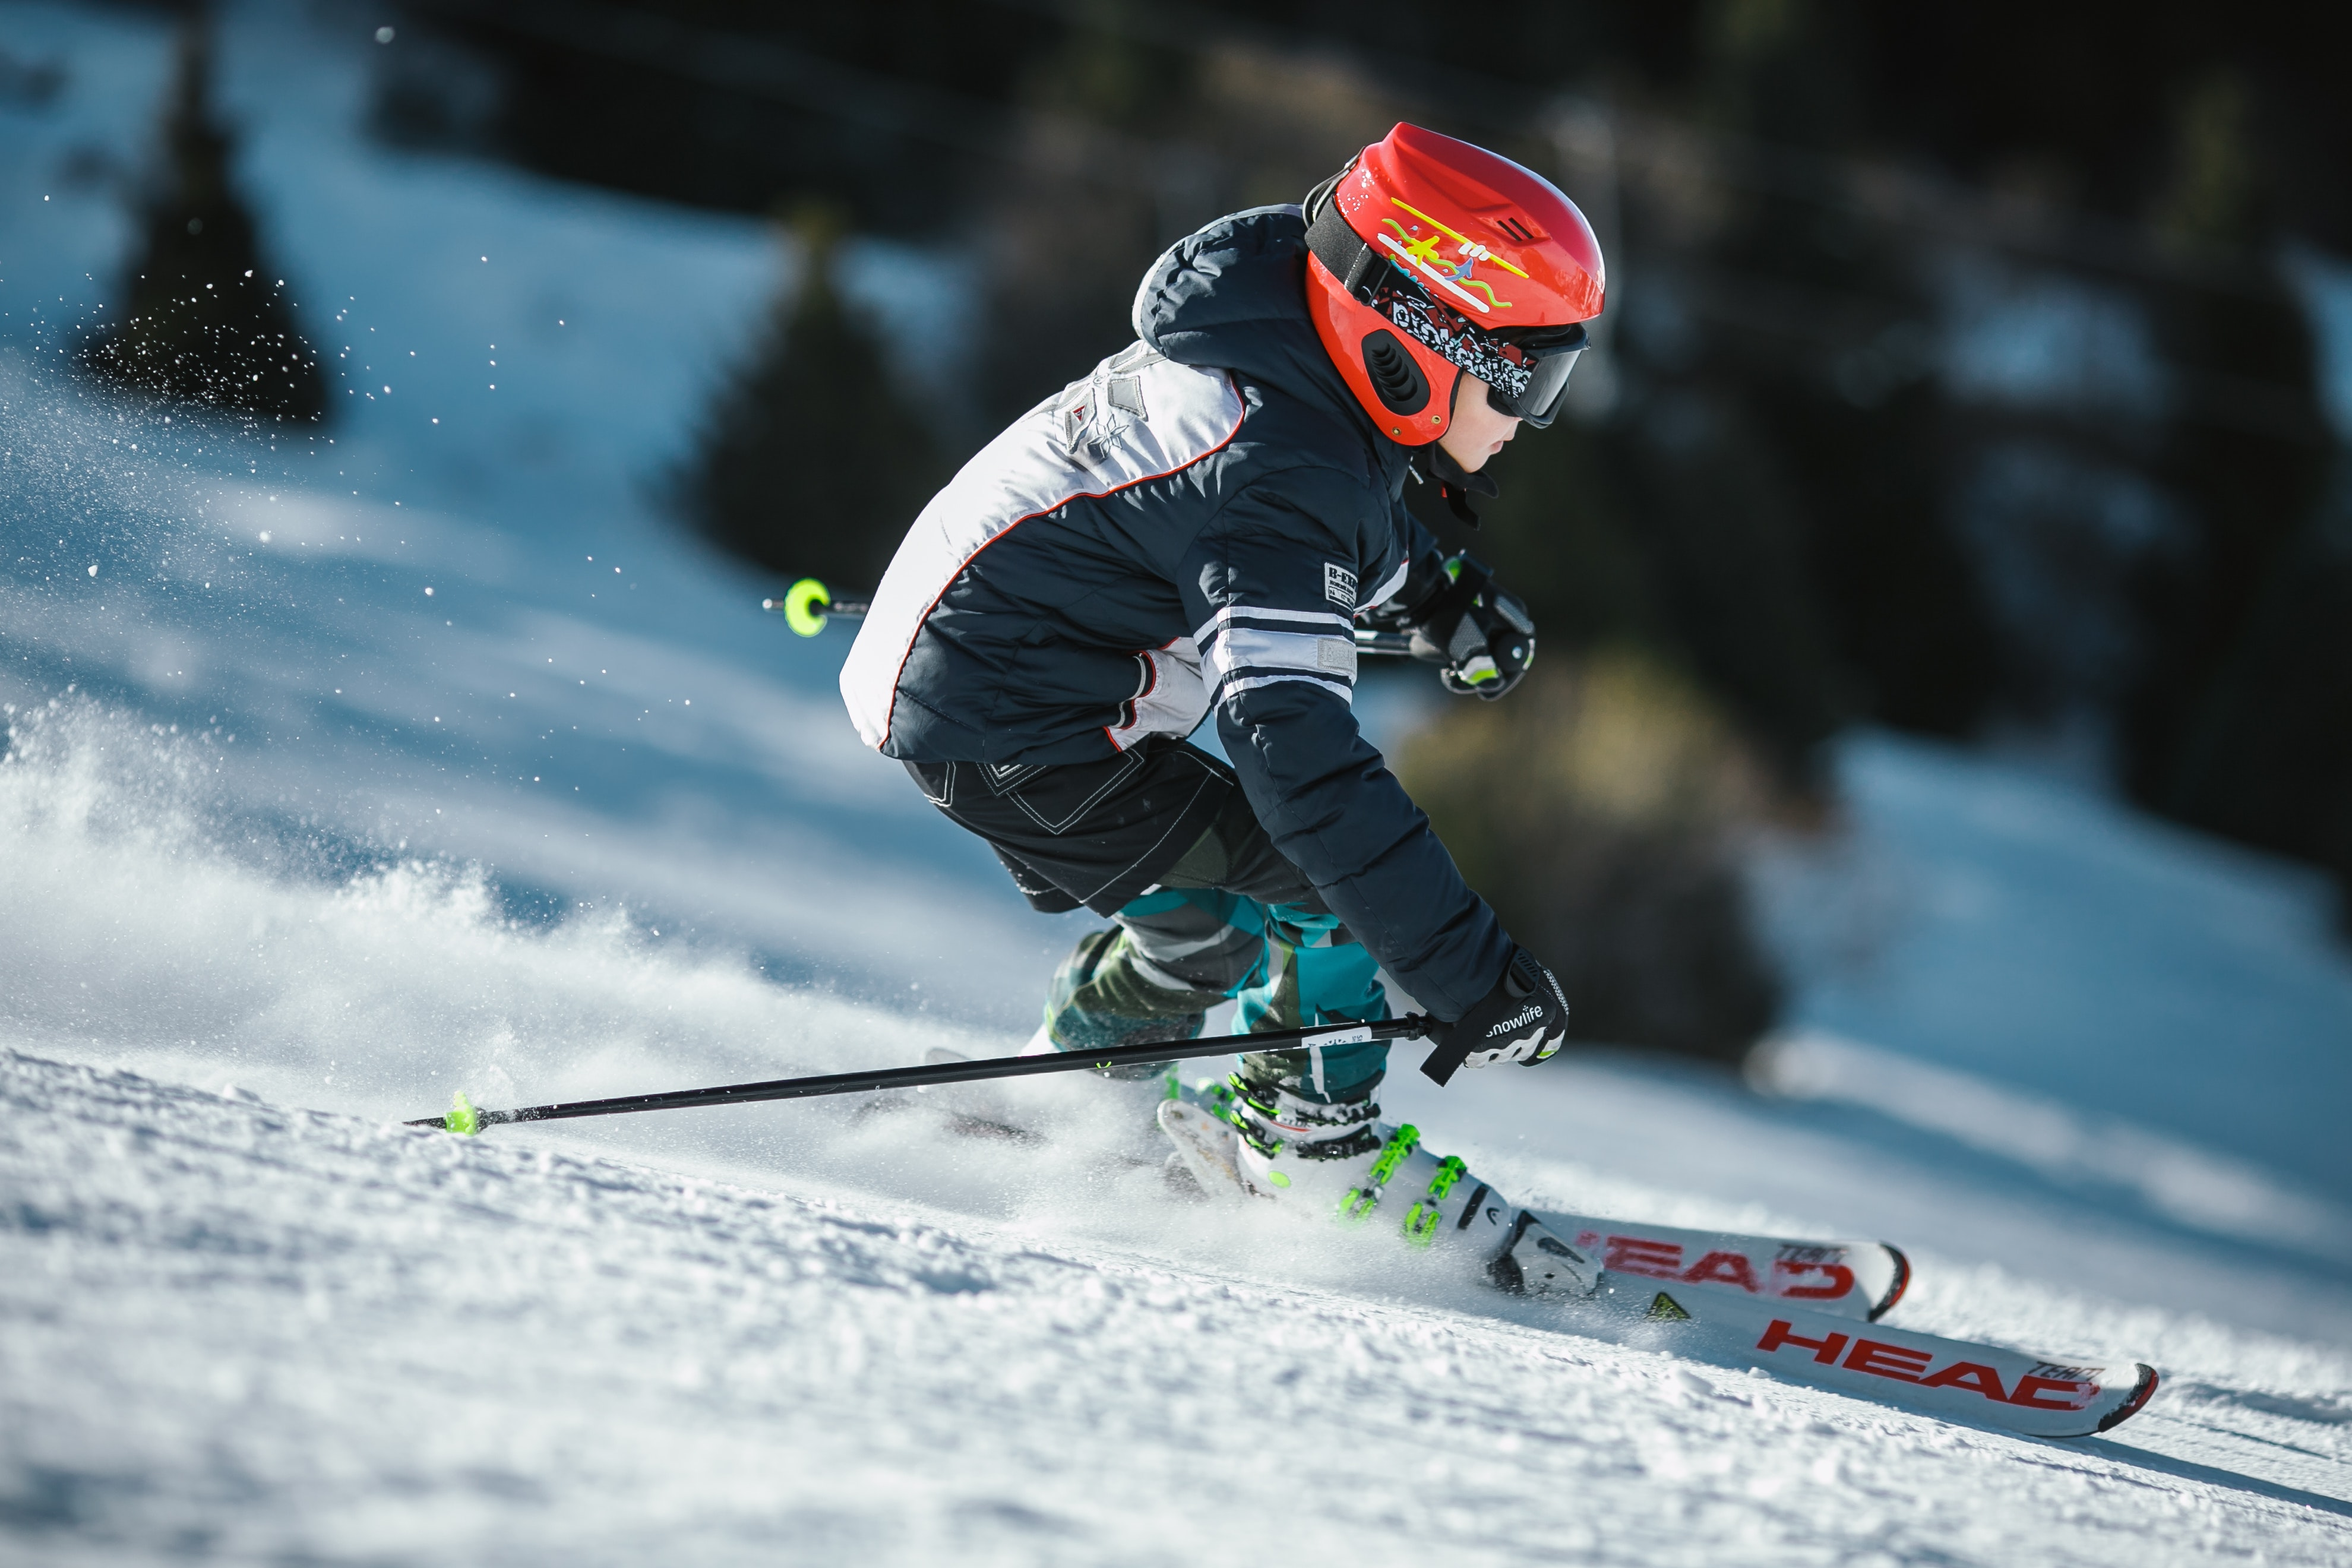
\includegraphics[width=1\linewidth]{medien/skifahrer.jpg}
				\caption[Nicht ich auf Skiern.]{Definitiv nicht ich. Zur Verfügung gestellt von: www.pexels.com/de-de/@visitalmaty/}
				\label{fig:skifahrer}
			\end{figure}
		\end{columns}
	\end{frame}
	\subsection{Optimierungsparameter}
	\begin{frame}
		\frametitle{Optimierungsparameter}
		\begin{itemize}
			\item{Kosten}
			\begin{itemize}
				\item{Leistungselektronik}
				\item{Batterie}
				\item{Optimierung des Wirkungsgrades}
			\end{itemize}
			\item{Nutzerfreundlichkeit}
			\begin{itemize}
				\item{Batterie soll den ganzen Tag lang halten}
				\item{Regelung möglichst einfach gestalten}
			\end{itemize}
		\end{itemize}
	\end{frame}
	\section{Lösungsansätze}
	\subsection{Widerstandsregler}
	\begin{frame}
		\frametitle{Widerstandsregler}
		\begin{columns}
			\column{0.5\textwidth}
			\begin{figure}[tbh]
				\centering
				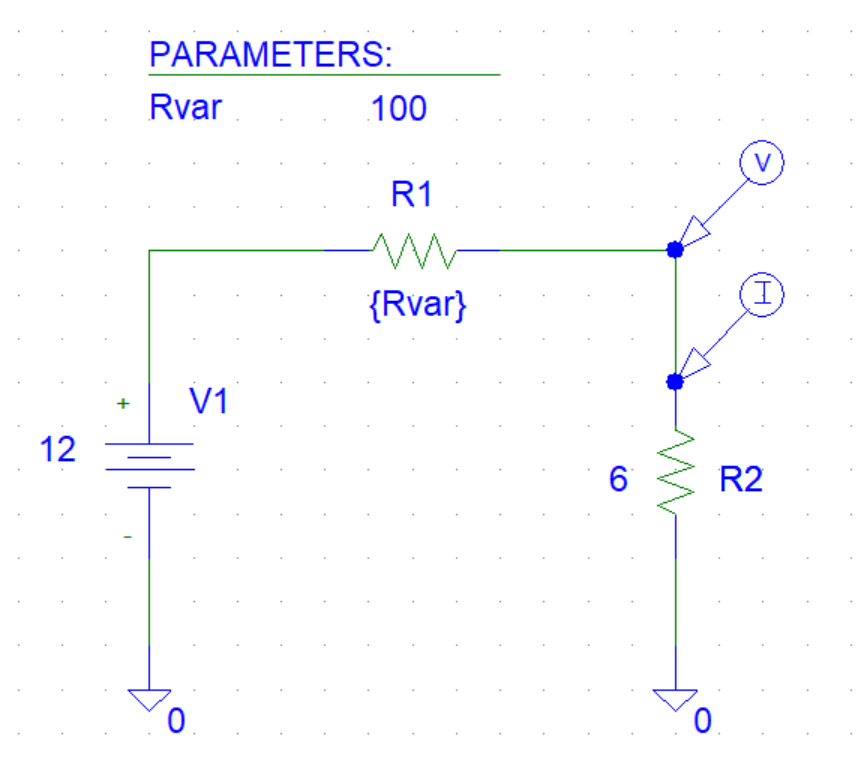
\includegraphics[width=1\linewidth]{medien/V1-0.png}
				\caption[Erster Aufbau]{Aufbau eines einfachen Spannungsteilers als Leistungsregelung.}
				\label{fig:aufbau1}
			\end{figure}
			\column{0.5\textwidth}
			\begin{itemize}
				\item{Einfache Leistungsanpassung}
				\begin{itemize}
					\item{z.B. durch Potentiometer}
					\item{Keine zusätzlichen Bauteile}
				\end{itemize}
				\item{Schlechter Wirkungsgrad}
				\begin{itemize}
					\item{Viel Leistung an R1}
				\end{itemize}
			\end{itemize}
		\end{columns}
	\end{frame}
	\begin{frame}
		\frametitle{Widerstandsregler}
		\begin{columns}
			\column{0.5\textwidth}
			\begin{figure}[tbh]
				\centering
				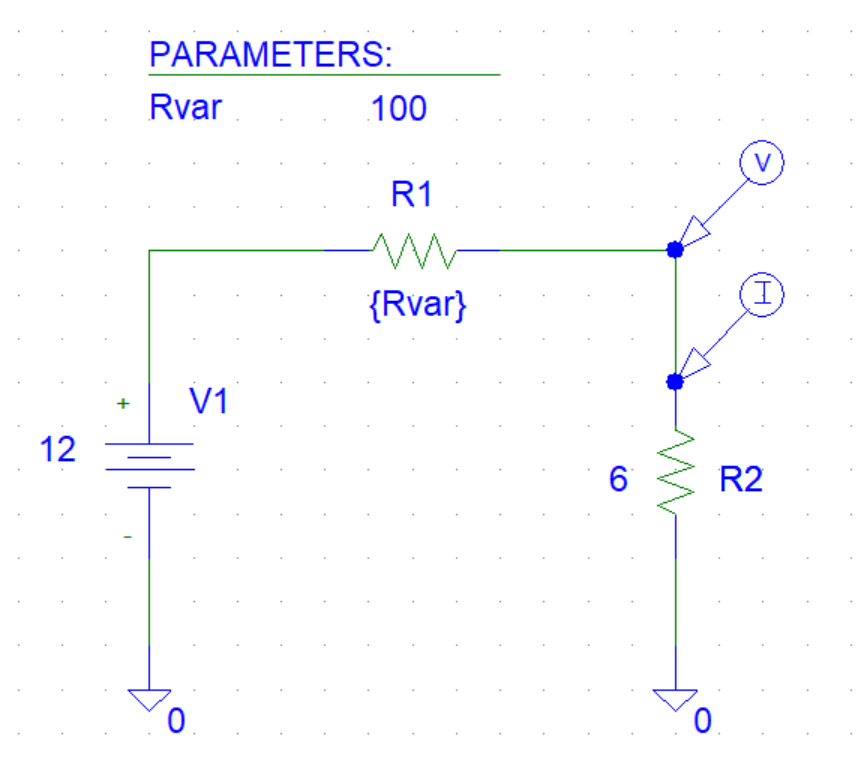
\includegraphics[width=1\linewidth]{medien/V1-0.png}
				\caption[Erster Aufbau]{Aufbau eines einfachen Spannungsteilers als Leistungsregelung.}
			\end{figure}
			\column{0.5\textwidth}
			\begin{align*}
				R_{ges}&=R_1+6\,\Omega \\
				I_{ges}&=\frac{12\, V}{R_{ges}} \\
				P_{heiz}=I_{ges}^2R_2&=12\, V\frac{6\,\Omega}{\left( R_1 + 6\,\Omega\right) ^2} \\
				P_{verlust}=I_{ges}^2R_1&=12\, V\frac{R_1}{\left( R_1 + 6\,\Omega\right) ^2} \\
				\eta &= \frac{P_{heiz}}{P_{heiz}+P_{verlust}}
			\end{align*}
		\end{columns}
	\end{frame}
	\begin{frame}
		%\frametitle{Widerstandsregler}
		\begin{center}
		\begin{figure}[tbh]
			\centering
			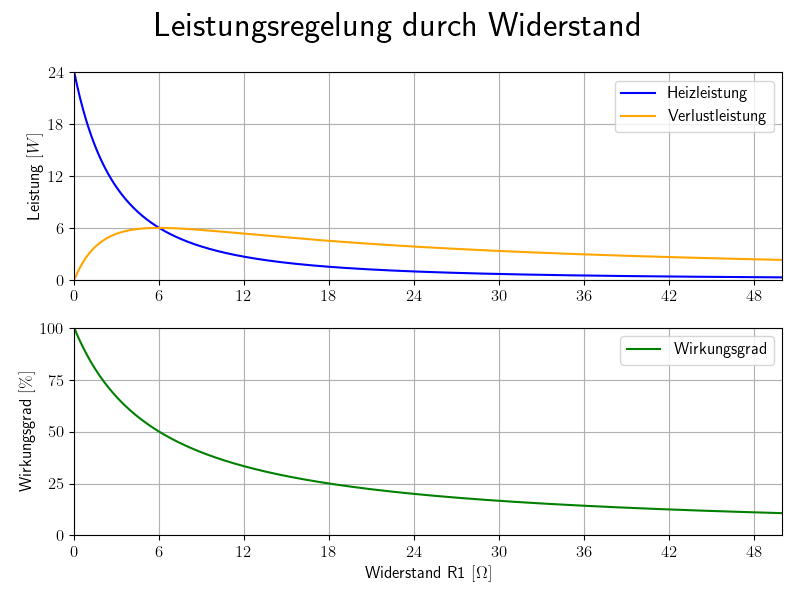
\includegraphics[width=0.95\linewidth]{medien/1.png}
			%\caption[Wirkungsgrad des ersten Aufbaues]{Wirkungsgrad des ersten Aufbauen über dem Widerstand $R_1$.}
			\label{fig:wirkungsgrad1}
		\end{figure}
		\end{center}
	\end{frame}
	\subsection{Operationsverstärker}
	\begin{frame}
		\frametitle{Operationsverstärker (OPV)}
		\begin{center}
			\begin{figure}[tbh]
				\centering
				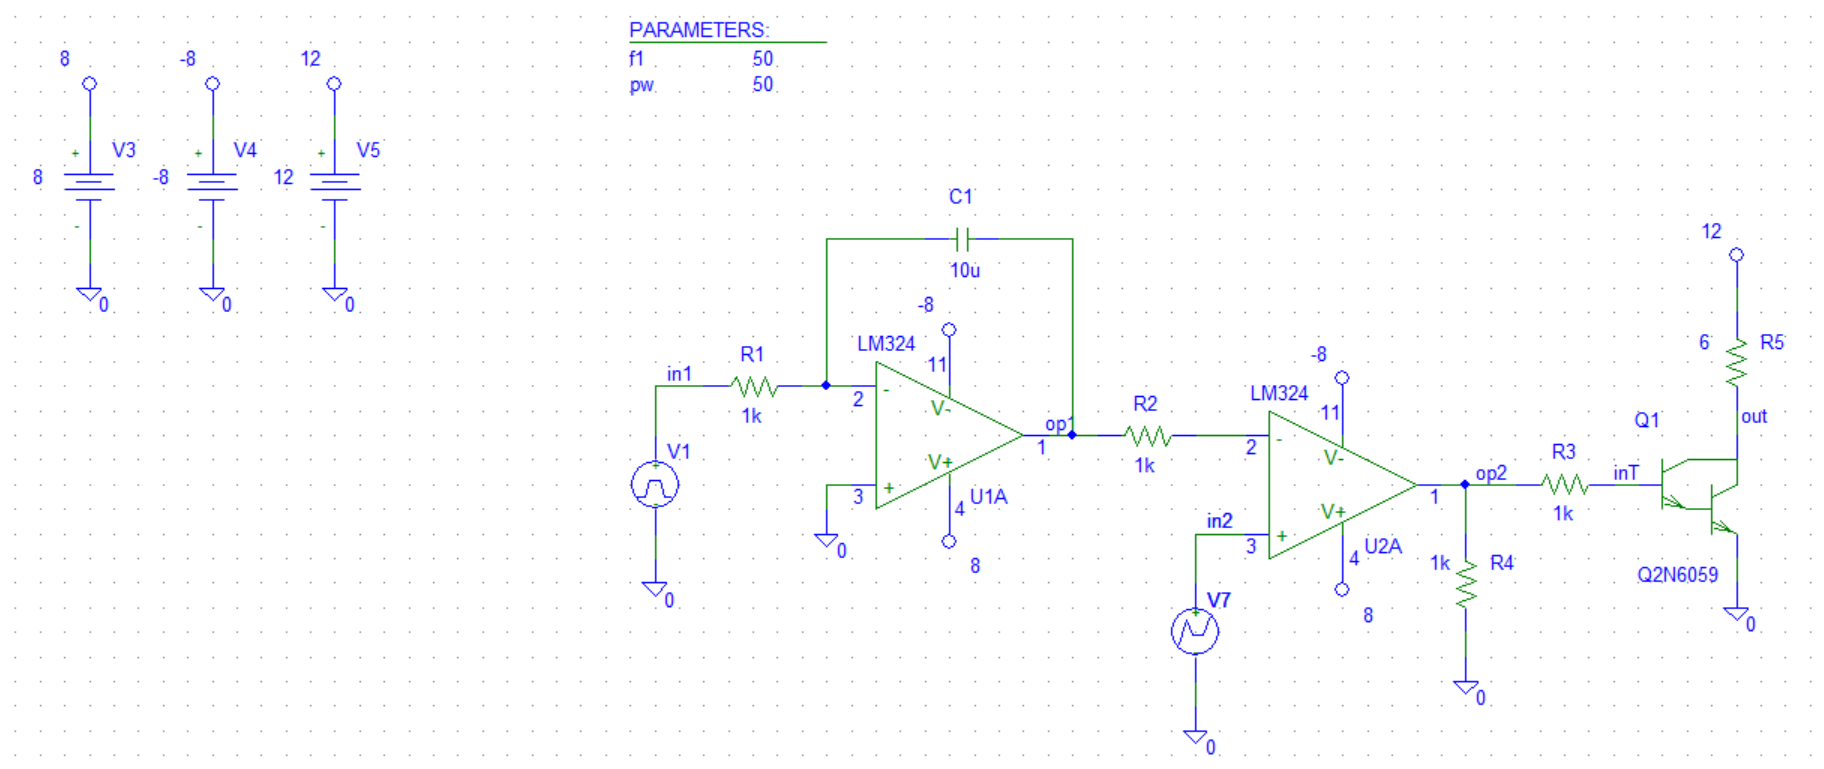
\includegraphics[width=0.95\linewidth , trim={10cm 0 0 0}]{medien/V2-0.png}
				\caption[Zweiter Aufbau]{Aufbau mit Operationsverstärkern als Leistungsregelung.}
				\label{fig:aufbau2}
			\end{figure}
		\end{center}
	\end{frame}
	\begin{frame}
		\frametitle{Operationsverstärker (OPV)}
		\begin{columns}
			\column{0.5\textwidth}
			\begin{figure}[tbh]
				\centering
				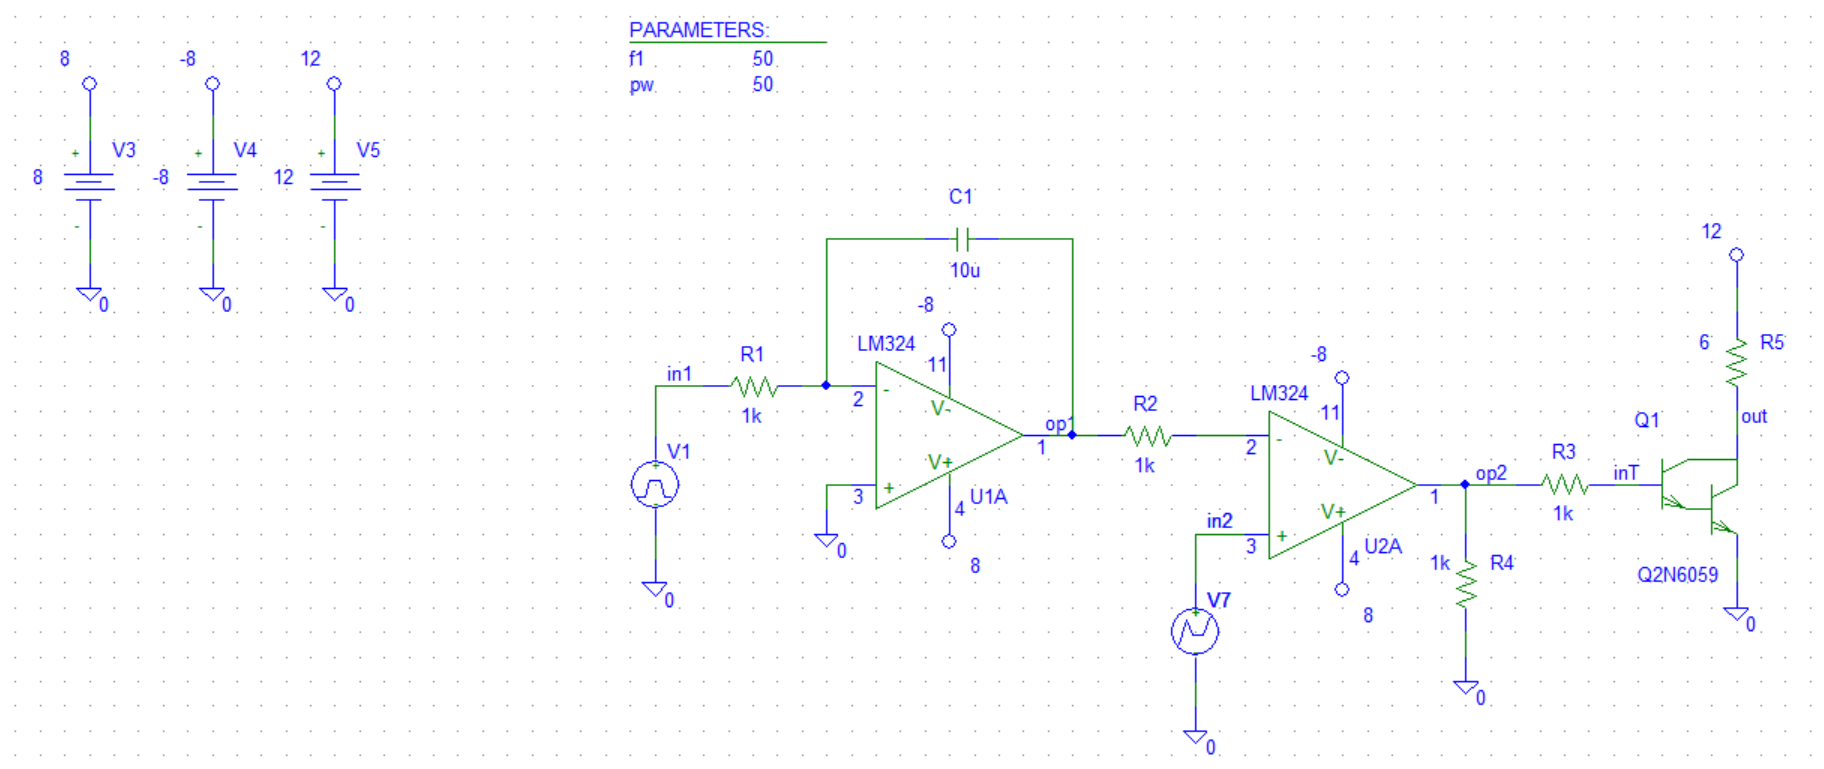
\includegraphics[width=1\linewidth , trim={10cm 0 0 0}]{medien/V2-0.png}
				\caption[Zweiter Aufbau]{Aufbau mit Operationsverstärkern als Leistungsregelung.}
			\end{figure}
			\column{0.5\textwidth}
			\begin{itemize}
				\item{Präzise Leistungsanpassung}
				\begin{itemize}
					\item{Ausgangsleistung linear von Schwellspannung abhängig}
				\end{itemize}
				\item{Hoher Wirkungsgrad}
				\begin{itemize}
					\item{Leistung der OPV verschwindend klein}
				\end{itemize}
			\end{itemize}
		\end{columns}
	\end{frame}
	\begin{frame}
		\frametitle{Operationsverstärker (OPV)}
		\begin{columns}
			\column{0.5\textwidth}
			\begin{figure}[tbh]
				\centering
				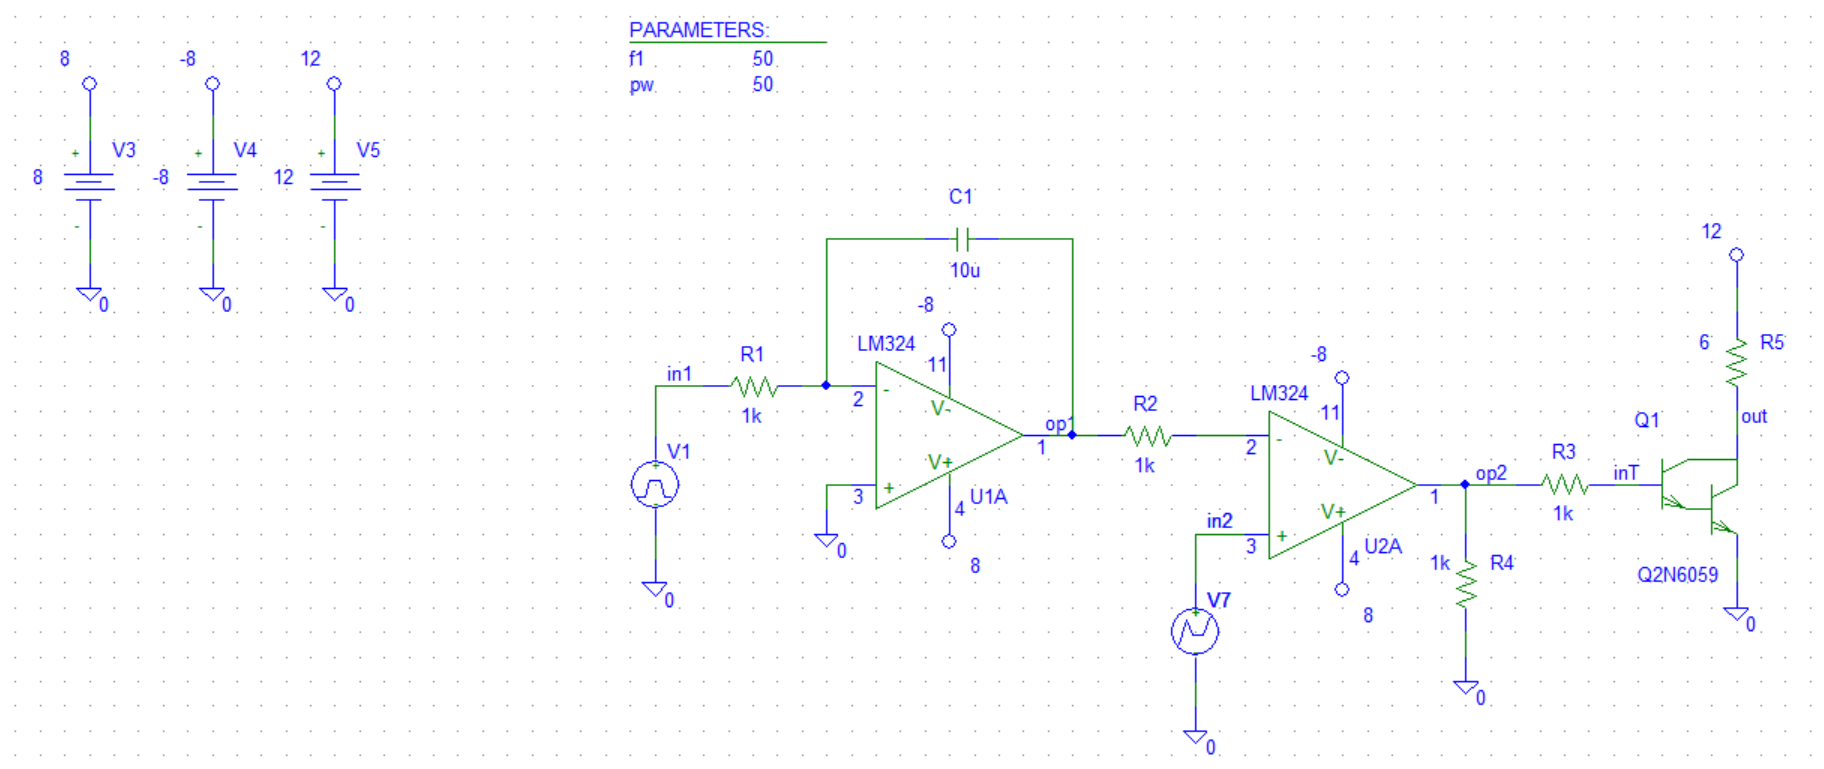
\includegraphics[width=1\linewidth , trim={10cm 0 0 0}]{medien/V2-0.png}
				\caption[Zweiter Aufbau]{Aufbau mit Operationsverstärkern als Leistungsregelung.}
			\end{figure}
			\column{0.5\textwidth}
			\begin{equation*}
				P_{heiz}=U_{R5}I_{R5}
			\end{equation*}
			Vereinfacht gilt
			\begin{equation*}
				P_{verlust}=U_{Q1_{ds}}I_{R5}
			\end{equation*}
			und daraus folgt
			\begin{equation*}
				\eta=\frac{P_{heiz}}{P_{heiz}+P_{verlust}}
			\end{equation*}
			für eine Einschaltdauer(\underline{d}uty \underline{c}ycle) von $dc \gg 0\,\%$
		\end{columns}
	\end{frame}
	\begin{frame}
		\begin{center}
			\begin{figure}[tbh]
				\centering
				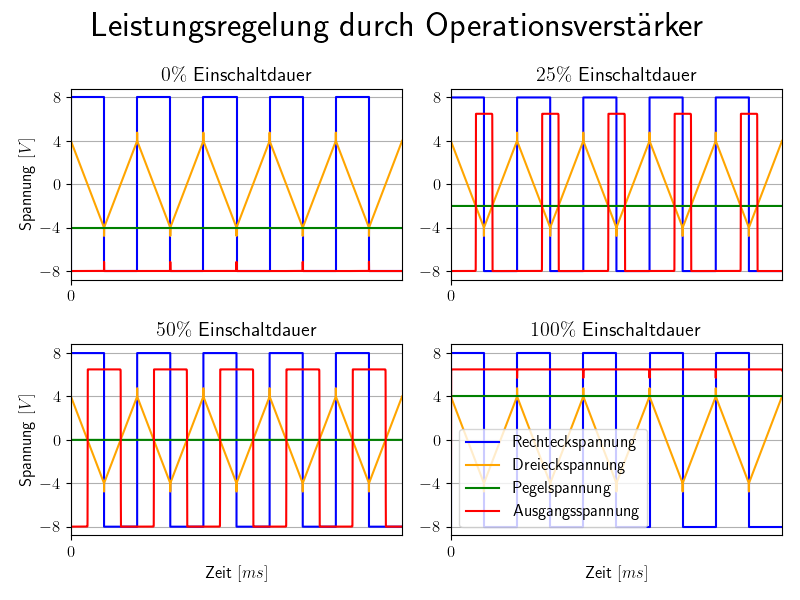
\includegraphics[width=0.95\linewidth]{medien/2.png}
				%\caption[Signalverlauf von Aufbau 2]{Signalverlauf von Aufbau 2 bei verschiedenen Einschaltdauern.}
			\end{figure}
		\end{center}
	\end{frame}
	\begin{frame}
		\frametitle{Verlustleistungen im Aufbau 2}
		\begin{center}
			\begin{figure}[tbh]
				\centering
				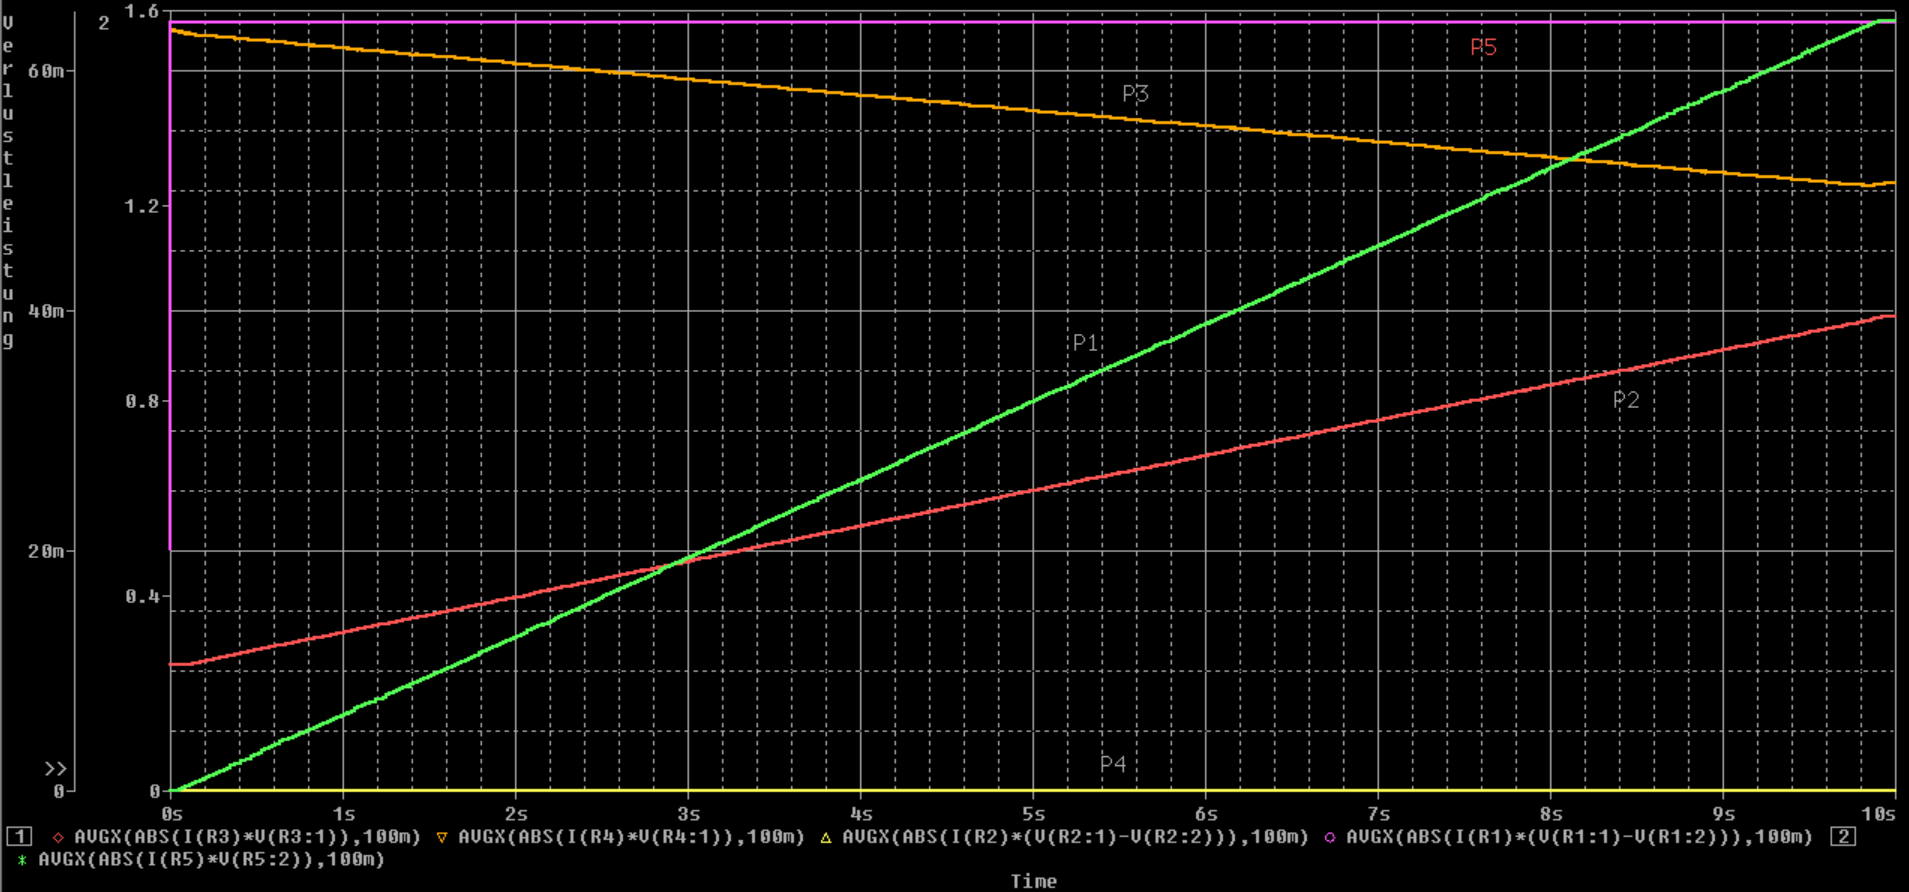
\includegraphics[width=1\linewidth]{medien/V2-3.png}
				\caption[Verlustleistungen Aufbau 2]{Verlustleistungen im Aufbau 2 über der Einschaltdauer. Legende:~\color{green}~$P_{Q1_{ds}}$,~\color{red}~$P_{R3}$,~\color{orange}~$P_{R4}$,~\color{yellow}~$P_{R2}$,~\color{magenta}~$P_{R1}$}
			\end{figure}
		\end{center}
	\end{frame}
	\subsection{Verbesserungsvorschlag}
	\begin{frame}
		\frametitle{Verbesserungsvorschlag}
		\begin{center}
			\begin{figure}[tbh]
				\centering
				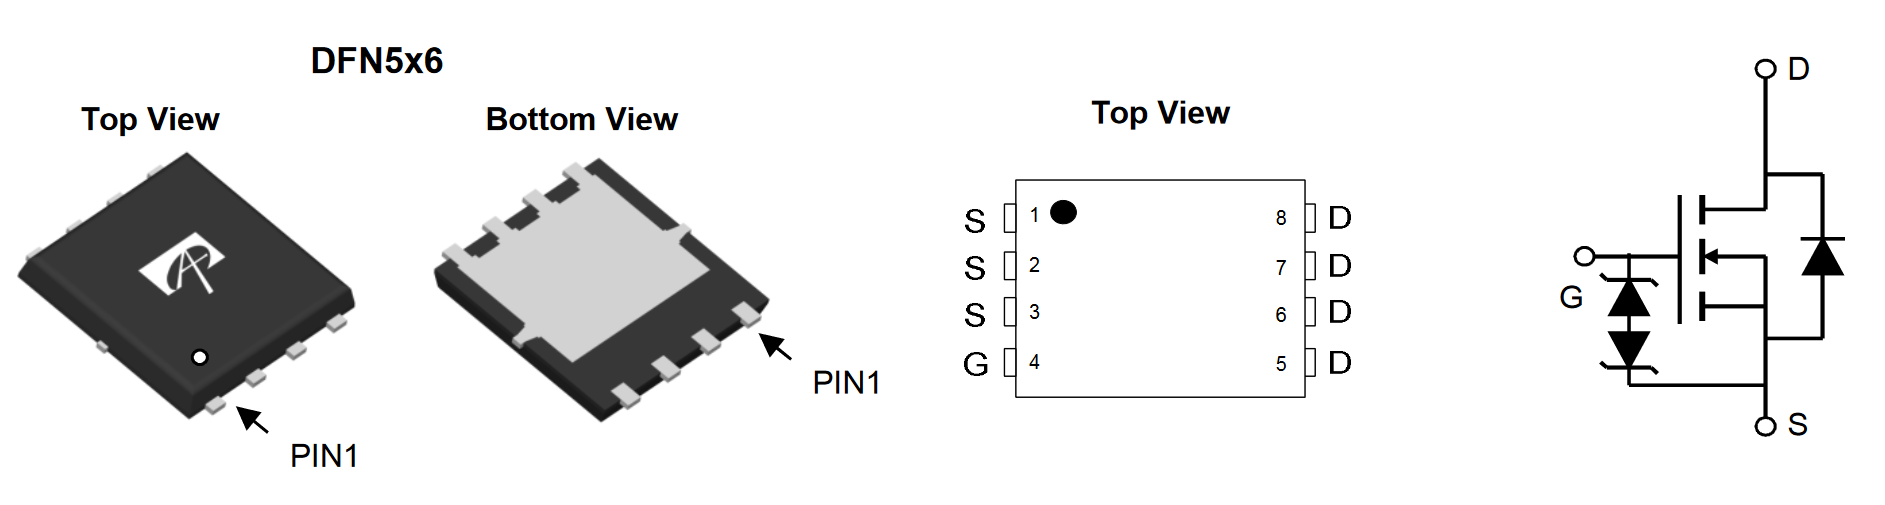
\includegraphics[width=1\linewidth]{medien/V3-4.png}
				\caption[MOSFET]{Leistungs MOSFET (AON6266E) für besseren Wirkungsgrad.}
			\end{figure}
		\end{center}
		\begin{itemize}
			\item{Wirkungsgrad}
			\begin{itemize}
				\item{$P_{R3} \approx 0$ (Geringe Leistung am Gate)}
				\item{$P_{Q2_{ds}} \ll P_{Q1_{ds}}$}
			\end{itemize}
			\item{Kosten bei Stückzahl 3000: $0,20876\,$\euro}
		\end{itemize}
	\end{frame}
	\section{Auswertung}
	\subsection{Vergleich der Ansätze}
	\begin{frame}
		\begin{center}
			\begin{figure}[tbh]
				\centering
				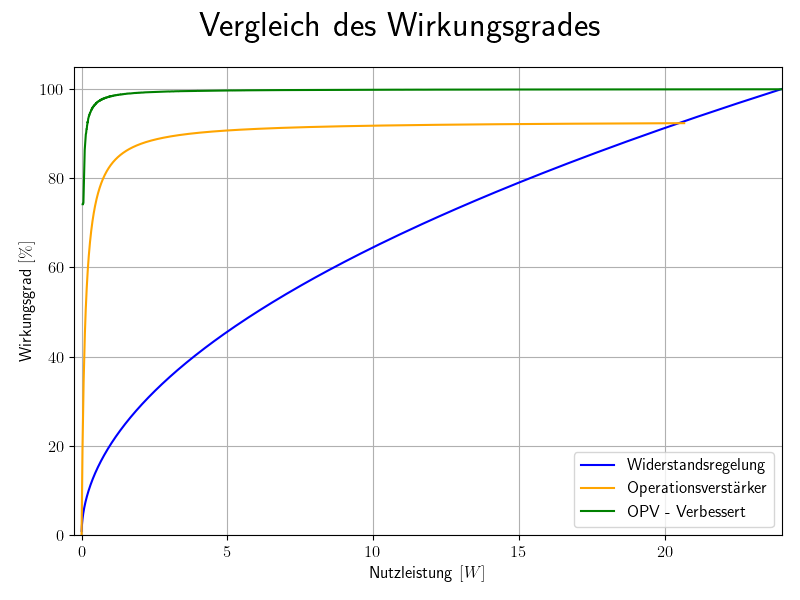
\includegraphics[width=0.95\linewidth]{medien/3.png}
			\end{figure}
		\end{center}
	\end{frame}
	\subsection{Fazit}
	\begin{frame}
		\frametitle{Fazit}
		\begin{columns}
			\column{0.3\textwidth}
			\textbf{Potentiometer}
			\begin{itemize}
				\item{Schlechter Wirkungsgrad}
				\item{Unwirtschaftlich}
			\end{itemize}
			\column{0.34\textwidth}
			\textbf{Operationsverstärker}
			\begin{itemize}
				\item{Konstanter Wirkungsgrad}
				\item{Günstig}
			\end{itemize}
			\column{0.33\textwidth}
			\textbf{OPV mit MOSFET}
			\begin{itemize}
				\item{Bester Wirkungsgrad}
				\item{Am günstigsten}
			\end{itemize}
		\end{columns}
	\end{frame}
	\begin{frame}
		\begin{center}
			\textbf{\Huge Viel Aufmerksamkeit für Ihren Dank!}
			
			Projekt: \url{https://www.github.com/stienek/pspice-abschlussprojekt}
		\end{center}
	\end{frame}
\end{document}